\documentclass[solution, letterpaper]{cs20inclass}
\usepackage{enumerate}
\usepackage{tikz}
\usepackage{pgf}
\usepackage{tikz}
\usepackage{hyperref}
\usepackage{ dsfont }
\usepackage{amsmath}
\begin{document}
\header{16}{Friday, March 04, 2016}

\noindent Author: Ben Zheng, Crystal Chang

\paragraph*{Executive Summary}

%% PROBLEM 1 %%
\problem We have a puzzle look like the following graph. What's the size of the state space after 2 moves?
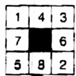
\includegraphics[width=2cm]{initial}

\begin{solution}
The size of the state space is 8.\\
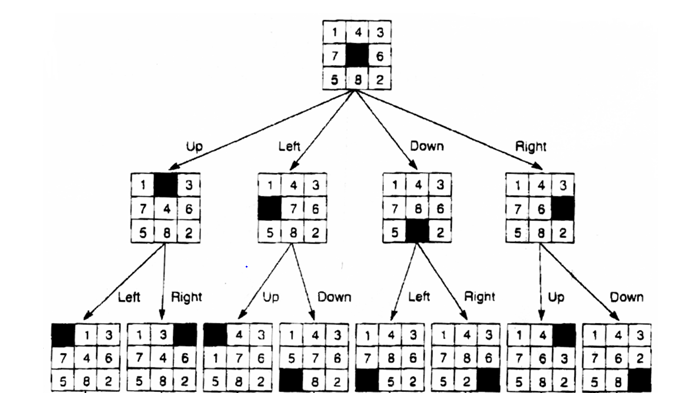
\includegraphics[width=12cm]{final8}
\end{solution}

%% PROBLEM 2 %%
\problem Use loop invariant to prove correctness property that y=c ($c>0$)after the following loop terminates.
\begin{itemize}
\item x=c; y=0;
\item while ($x>0$):
\subitem $x--$
\subitem $y++$
\end{itemize}
\subproblem Construct a loop invariant for the proof.
\subproblem Use induction to prove that the loop preserves the invariant.
\subproblem Use loop invariant to prove correctness property that y=c ($c>0$)after loop terminates.

\begin{solution}
\subsolution
\begin{itemize}
\item Let state set S=$N*N*N$: the values of (x, y, c)
\item $(x,y,c) \rightarrow (x-1, y+1, c)$  in each iteration of loop.
\item Let $P(x,y,n)\equiv$''x+y=c'' 
\item $y++$
\end{itemize}
\subsolution
\begin{itemize}
\item Base case: loop invariant x+y=c+0=c $\rightarrow$ P(c,0,c) holds.
\item Induction step: \\
Assume loop invariant holds after k iterations:\\
x=c-k; y=k;\\
after the (k+1) th iteration, y=k+1, x=c-k-1\\
And x+y=k+1+c-k-1=c\\
Therefore, the loop preserves the invariant P(x,y,n).
\end{itemize}
\subsolution
After final iteration: x=0;\\
we also know our loop invariant holds: x+y=c. Therefore, y=c.
\end{solution}

%% PROBLEM 3 %%
\problem Consider the following piece of code $(n>0)$:
\begin{itemize}
\item y=0; i=0
\item while ($i< n$):
\subitem $y += 2^i$
\subitem $i++$
\end{itemize}
\subproblem Compute the value of y after 0th,1th,2nd,3rd iteration and guess what would be the value of y after the loop termination?
\subproblem Take use of what you get in (A) to construct  a loop invariant.
\subproblem Use induction to prove that the loop preserves the invariant.
\subproblem Use loop invariant to prove correctness property that y=c ($c>0$)after loop terminates.

\begin{solution}
\subsolution
\begin{itemize}
\item iteration 0: $y_0=0=2^0-1$
\item iteration 1: $y_1=2^0=1=2^1-1$
\item iteration 2: $y_2=2^0+2^1=1+2=3=2^2-1$
\item iteration 3: $y_3=2^0+2^1+2^2=1+2+4=7=2^3-1$
\item iteration n: $y_n=2^0+2^1+2^2+...+2^{n-1}=2^n-1$
\end{itemize}
\subsolution
\begin{itemize}
\item Let state set S=$N*N*N$: the values of (y, i, n)
\item $(y,i,n) \rightarrow (y+2^i, i+1, n)$  in each iteration of loop.
\item Let $P(y, i, n)\equiv y=2^i -1$ 
\end{itemize}
\subsolution
\begin{itemize}
\item Base case: i=0: $y_0=0=2^0-1$ $\rightarrow$ P(0,0,n) holds.
\item Induction step: \\
Assume that at the start of the k-th iteration $y_k=2^k-1$\\
Then, at the start of the (k+1)-th iteration we will have:\\
$y_{k+1}=y_k+2^k=2^k-1+2^k=2*2^k-1=2^{k+1}-1$ Q.E.D.
\end{itemize}
\subsolution
When the loop terminates i=n. Thus after the loop execution we have: $y=2^{n}-1$
\end{solution}


%% PROBLEM 4%%


\end{document}